\section{Reference inference and implementation details}
\label{app:reference}

\subsection{The oracle and the fitted Gaussian reference}

The oracle uses the actual parameters of the synthetic deployment. It conditions on the observed sensor subset under that deployment and therefore measures performance with task uncertainty removed. Its role is diagnostic. It shows whether an inference mechanism loses information even when its sensor model is known, and it supplies a lower risk reference under the specified generator.

FA Gaussian instead estimates its parameters from the incomplete support. The network anchor uses eight EM iterations, whereas the reported closed form reference uses forty. Both fit the joint Gaussian before extracting the factor structure. The stronger closed form reference is not numerically identical to the initial network in every episode. This distinction matters when interpreting the gain from learning: the final network is compared against the specified reference, rather than against a deliberately identical numerical starting point.

The reported EM Gaussian, FA Gaussian and ridge references inflate predictive variance by \(n/(n-|S|-1)\). This is part of the reference implementation, not a consequence of the exact site identity. The learned models predict their own corrected variances. Comparisons therefore evaluate the complete specified predictors, including their treatment of finite support uncertainty.

\subsection{The sign conditioned sampling reference}

The sampling reference approximates inference over the synthetic task parameters from the support, using the generator prior~\citep{neal2011hmc}. There are \(5P\) parameters, or twenty five in the main setting. The shared nuisance is integrated analytically through a covariance that is diagonal plus rank one. Only observed calibration entries contribute to each row's likelihood.

The response sign of each sensor is fixed using its support correlation. The generator's lower bound on response magnitude does not guarantee that the sign is recovered from every finite support set. Fixing it reduces the posterior being sampled and omits uncertainty over alternative signs. For this reason, the reference is called sign conditioned HMC throughout the manuscript. It is a useful numerical comparison, rather than a certified Bayes optimal ceiling for the full task prior.

The implementation uses four chains per task, each initialized from a maximum a posteriori fit. Warmup first adapts step size toward an acceptance probability of \(0.75\), estimates a diagonal mass matrix over one hundred and fifty iterations, and then performs one hundred and fifty further adaptation iterations. Fifty retained draws per chain are thinned by a factor of four, with twelve leapfrog steps per trajectory.

Let \(\theta^{(b)}\) denote a retained parameter draw. The predictive distribution includes the information in the query readings themselves:
\begin{equation}
 p(y\mid x_S,\D)
 \ \approx\
 \frac{\sum_b p(y,x_S\mid\theta^{(b)})}
 {\sum_b p(x_S\mid\theta^{(b)})}.
 \label{eq:hmc-predictive}
\end{equation}
The denominator is evaluated by trapezoidal quadrature on three hundred and one points. This query weighting differs from simply averaging \(p(y\mid x_S,\theta^{(b)})\) under the support posterior with equal weights. Query readings can make some deployment parameter draws more plausible than others.

Across the panels on which this reference was run, the recorded convergence diagnostic \(\widehat R\) was below \(1.1\) for at least \(99.9\%\) of identifiable parameters. A check with known generator parameters reproduces the exact oracle predictive calculation within \(2\times10^{-3}\) nats. These checks assess the implemented calculation and sampling behavior under the recorded setup. They do not eliminate finite Monte Carlo error or the response sign conditioning.

\subsection{Positive variance and Gaussian readout}

Each corrected noise variance multiplies a positive anchor variance by
\begin{equation}
 \exp\{4\tanh(s_j/4)\}.
\end{equation}
For finite network outputs this multiplier is positive and bounded between \(e^{-4}\) and \(e^4\). The construction prevents a negative measurement variance. The proper prior then keeps the joint precision positive definite in exact arithmetic. Implementations still require numerically stable linear algebra, especially when fitted sensor responses are large or the support covariance is nearly singular.

For \(d=1+K\), accumulating \(P\) dense rank one site contributions requires \(O(Pd^2)\) arithmetic. Solving the final \(d\) dimensional Gaussian system requires \(O(d^3)\) arithmetic with a conventional dense factorization. These expressions describe the readout after site construction. They omit support fitting, neural feature construction and any transformer attention, so they are not a total inference runtime claim. In the reported \(K=1\) setting the Gaussian state has two coordinates.

For cavity refinement, each site is removed from the sum before forming its update. Since the remaining precision is the prior plus positive semidefinite sites, it is positive definite in exact arithmetic. Updates are synchronous: every new site in a round uses cavities built from the previous round's sites. This avoids making the calculation depend on an arbitrary sensor update order. The original learned model nevertheless depends on the chosen nuisance coordinates, as the factor orientation audit makes clear.

\subsection{Training comparison}

The compact cavity model and the transformer are trained on the same synthetic task distribution and query mask rule, but their optimization recipes are not identical. The compact network draws from a finite task pool, whereas the transformer receives fresh tasks at every step. Their batch shapes, learning rates, clipping thresholds and step counts also differ. The primary compact versus transformer result therefore compares the specified complete training procedures. The transformer and transformer site model share a more closely matched backbone and recipe, making that comparison more informative about the effect of the output construction.

\begin{figure*}[t]
\centering
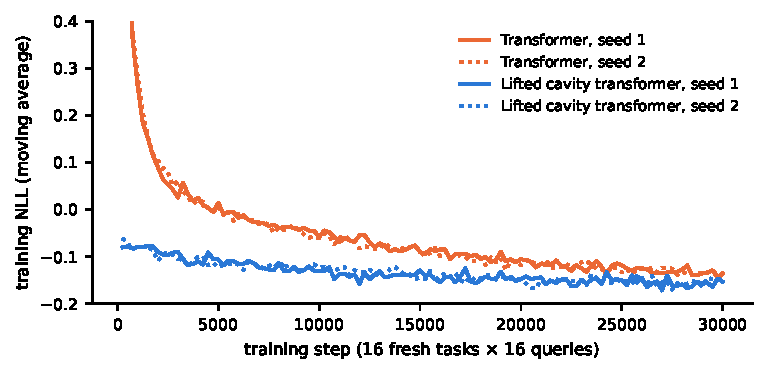
\includegraphics[width=.88\textwidth]{figures/historical_training.pdf}
\caption{\label{fig:training}Historical training likelihood curves for the transformer and its lifted site variant. Both use the same backbone, recipe and training seed in the recorded comparison. The site output starts at a fitted Gaussian anchor. The conventional output must first learn a predictor from its generic initialization. These curves are retained from the original score based paper export.}
\end{figure*}

The implementation registers the original transformer's generic output head inside its backbone, even when the lifted site model uses a separate site head for prediction. Registered parameter counts therefore include a small head that is not used by the lifted prediction route. This detail explains why the parameter count increases by the full additional site head rather than by the difference between two replacement heads.

The architecture figures are conceptual renderings of these computations. Their support matrices and sensor traces are illustrative, and their analytical sign reversal example follows the stated Gaussian model. They do not display newly collected sensor data or newly measured benchmark outcomes.
